\documentclass[border=8pt]{standalone}
\usepackage{amsmath,amssymb}
\usepackage{tikz}
\usetikzlibrary{arrows.meta, positioning}
\begin{document}
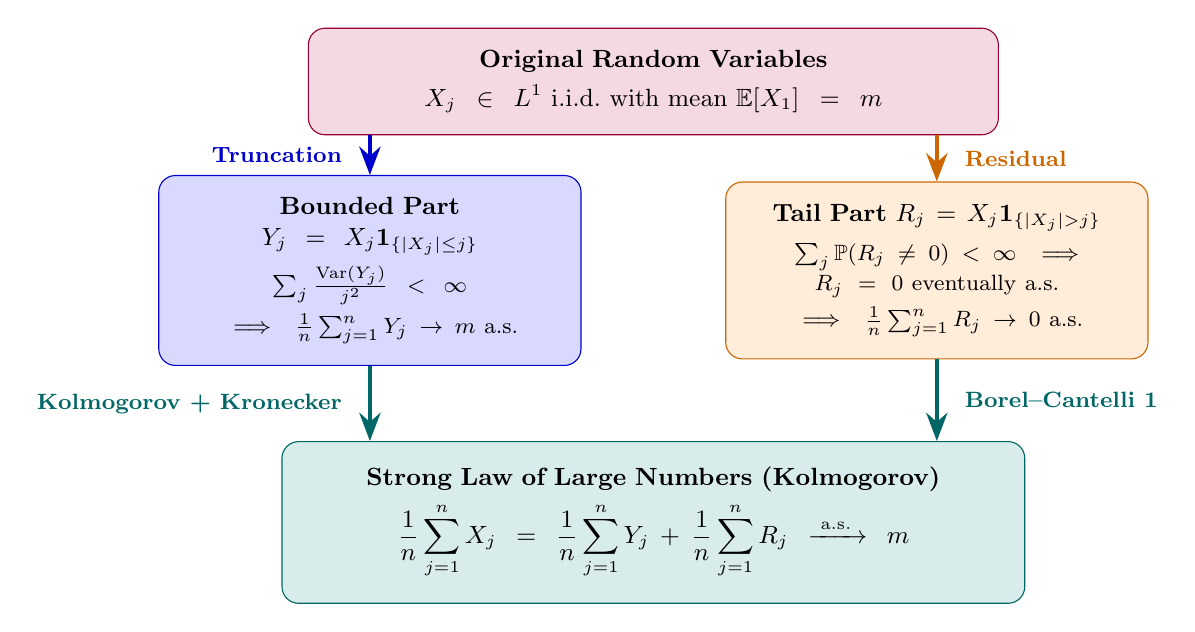
\begin{tikzpicture}[font=\small, >=Stealth]
  \node[draw=purple!80!black, rounded corners=6pt, fill=purple!15, text width=8.2cm, align=center, inner sep=8pt] (X) at (0, 3.8)
    {\textbf{Original Random Variables}\\[3pt] $X_j \in L^1$ i.i.d.\ with mean $\mathbb{E}[X_1] = m$};

  \node[draw=blue!80!black, rounded corners=6pt, fill=blue!15, text width=4.8cm, align=center, inner sep=8pt] (Y) at (-3.6, 1.4)
    {\textbf{Bounded Part} $Y_j = X_j \mathbf{1}_{\{|X_j| \le j\}}$\\[3pt]
     {\footnotesize $\sum_{j} \frac{\mathrm{Var}(Y_j)}{j^2} < \infty$}\\[2pt]
     {\footnotesize $\implies \frac{1}{n}\sum_{j=1}^n Y_j \to m$ a.s.}};

  \node[draw=orange!80!black, rounded corners=6pt, fill=orange!15, text width=4.8cm, align=center, inner sep=8pt] (R) at (3.6, 1.4)
    {\textbf{Tail Part} $R_j = X_j \mathbf{1}_{\{|X_j| > j\}}$\\[3pt]
     {\footnotesize $\sum_j \mathbb{P}(R_j \ne 0) < \infty \implies R_j = 0$ eventually a.s.}\\[2pt]
     {\footnotesize $\implies \frac{1}{n}\sum_{j=1}^n R_j \to 0$ a.s.}};

  \node[draw=teal!80!black, rounded corners=6pt, fill=teal!15, text width=8.8cm, align=center, inner sep=9pt] (SLLN) at (0, -1.8)
    {\textbf{Strong Law of Large Numbers (Kolmogorov)} \\[3pt]
     $\displaystyle \frac{1}{n} \sum_{j=1}^n X_j = \frac{1}{n} \sum_{j=1}^n Y_j + \frac{1}{n} \sum_{j=1}^n R_j \xrightarrow{\;\mathrm{a.s.}\;} m$};

  \draw[->, line width=1.6pt, blue!80!black] (X.south -| Y.north) -- (Y.north)
    node[midway, left=6pt, font=\footnotesize\bfseries, text=blue!80!black] {Truncation};
  \draw[->, line width=1.6pt, orange!80!black] (X.south -| R.north) -- (R.north)
    node[midway, right=6pt, font=\footnotesize\bfseries, text=orange!80!black] {Residual};

  \draw[->, line width=1.6pt, teal!80!black] (Y.south) -- (Y.south |- SLLN.north)
    node[midway, left=6pt, font=\footnotesize\bfseries, text=teal!80!black] {Kolmogorov + Kronecker};
  \draw[->, line width=1.6pt, teal!80!black] (R.south) -- (R.south |- SLLN.north)
    node[midway, right=6pt, font=\footnotesize\bfseries, text=teal!80!black] {Borel--Cantelli 1};
\end{tikzpicture}
\end{document}
